In this section, we discuss previous approaches to NLG, including
the two main diverging approaches.  Broadly, these are the
approaches utilizing statistical generation and classical planning,
respectively.  We discuss these two branches in terms of their
exemplar systems, Halogen \cite{langkilde_2002_halogen}
and CRISP \cite{koller_sentence_2007}, respectively.
We also discuss prior work in dialog systems,
which represent an application of NLG to
real-world problems.

\section{Approaches to NLG}
Two broad categories of
approaches have been used to attack the general NLG problem. One
direction can be thought of as ``overgeneration and ranking.'' Here
some (possibly probabilistic) structure is used to generate multiple
candidate sentences, which are then ranked according to how well they
satisfy the generation criteria. This includes work based on chart
generation and
parsing~\cite{shieber_uniform_1988,kay_chart_1996}. These generators
assign semantic meaning to each individual token, then use a set of
rules to decide if two words can be combined.  Any combination which
contains a semantic representation equivalent to the desired meaning 
is a valid output from a chart generation
system.

A second line of attack formalizes NLG as an AI planning problem.
SPUD \cite{stone_2003_spud}, a system for NLG which uses planning,
considers NLG as a problem which requires realizing a deliberative
process of goal-directed activity.  Many such NLG-as-planning systems
use a pipeline architecture, working from their communicative goal
through a series of processing steps and concluding by outputting the
final sentence in the desired natural language. This is usually done
into two parts:
discourse planning and sentence generation. In
discourse planning, information to be conveyed is selected and split
into sentence-sized chunks. These sentence-sized chunks are then sent
to a {\em sentence generator}, which itself is usually split into two
tasks, {\em sentence planning} and {\em surface realization}
\cite{koller_experiences_2011}.  The sentence planner takes in a
sentence-sized chunk of information to be conveyed and enriches it in
some way, often by adding semantic annotations.  
This is then used by a {\em surface realization}
module which encodes the enriched semantic representation into 
 natural language.  This chain is sometimes referred to as the
``NLG Pipeline'' \cite{reiter_building_2000}.  Our approach is
part of this broad category.

A subcategory of this approach, called {\em integrated generation}, considers both
sentence generation portions of the pipeline together.
\cite{koller_sentence_2007}.  This is the approach taken in some
modern generators like CRISP \cite{koller_sentence_2007} and PCRISP
\cite{bauer_sentence_2010}.  In these generators, the input semantic
requirements and grammar are encoded in PDDL~\cite{fox2003pddl2},
which an off-the-shelf classical planner such as
Graphplan~\cite{blum_1997_graphplan} uses to produce a list of
applications of rules in the grammar.  These generators generate
parses for the sentence at the same time as the sentence, which keeps
them from generating realizations that are grammatically incorrect,
and keeps them from generating grammatical structures that cannot be
realized properly. PCRISP extends CRISP by adding support for
probabilistic grammars. However the planner in PCRISP's back end is
still a standard PDDL planner, so PCRISP transforms the probabilities
into costs so that a low likelihood transition has a high cost in
terms of the plan metric.

\subsection{Halogen / Nitrogen}

The exemplar system for the statistical generation approach is the
Halogen / Nitrogen family of systems, based on the idea of
ranking thousands of sentences based purely on syntactic probability,
using a special data structure called a "word lattice".
A word lattice can be thought of as a DAG where each edge is
labeled with a single word.  The DAG is constructed such that
any path from a specially labeled start node to a specially labeled
end node is a valid English sentence (at least between adjacent nodes).
This data structure enables the calculation of sentence likelihoods
(the probability that an arbitrary sentence chosen from a grammar
learned from a corpus would match this sentence), and the many
sentences which can be generated
given syntactic unknowns can be ranked efficiently.

Systems like these take a semantic input like that shown in
the appendix figure \ref{halogen-example}.  This input
has the advantage of being relatively easy for humans to
read, but relatively difficult for machines to create.
However, these systems are very efficient and able
to produce desirable outputs in many cases.  Due to
their structure, they are only truly able to consider local
dependencies of very short length.  In fact, the
initial version of Halogen worked on a bigram model
and generated sentences like "I only hires men who is good 
pilots." \cite{knight_1995_genselect}.  Obviously, the
linguistic model of combining words and choosing the most likely
ordering will not always generate sentences which accomplish
the desired linguistic goal, and requires eliminating all
sentences which do not accomplish the linguistic goal
before generation even begins.  Later work on these
generators included the scoring of the top
sentences by more expensive and reliable means, which
improved generation quality substantially at the cost of
little time. \cite{langkilde1998generation}

Fundamentally, these systems have the advantage of
fast and linguistically plausible generation.  They
take advantage of Zipf's Law, which causes them
to be fairly reliable under certain conditions.  When
those conditions are not met, however, the generators perform
badly; with no real understanding of their output, they
cannot adequately correct for bad entries in their word
lattice.

\subsection{CRISP / PCRISP}

CRISP is the exemplar system of the planning approach to NLG.
CRISP treats the problem of generation as a classical planning
problem; the goal state is any state in which the sentence
currently being generated matches the desired meaning.
Actions add new words to the sentence, and consequently
modify CRISP's representation of the meaning of the sentence.
This means that CRISP needs to keep a representation of the
way in which every entry in the grammar it uses changes the
meaning of any sentence in which it is placed.
CRISP uses LTAGs as its grammar formalism,
which means that these meanings will be phrased as components
of tree-rewrite rules.  For example, see Figure \ref{crisp-grammar},
originally published in \cite{koller_experiences_2011}.
This can be problematic for some generation problems, but works well
for simple sentences.

\begin{figure}
\centering
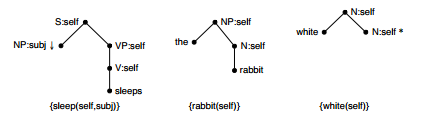
\includegraphics{crisp-grammar.png}
\caption{An example CRISP grammar.  Note the semantic annotations
beneath each tree.}
\label{crisp-grammar}
\end{figure}

CRISP uses Graphplan to search for a solution to the planning
problem which describes its generation problem.  This has
the advantage of running very quickly on some types of
sentences.  It also has the advantage of ignoring irrelevant
pieces of the grammar automatically, reducing the number
of states that need to be considered substantially.
It is also a complete search; if a solution to the generation
problem exists using the grammar and lexicon CRISP is provided,
CRISP will never fail to find it.

PCRISP \cite{bauer_sentence_2010} is a later improvement to
CRISP which attempts to address the inability of CRISP to consider
probabilities in its generation.  PCRISP's core advancement is
to perform its planning by searching the most probable sentences
first.  This combines, in some sense, the Halogen / Nitrogen model
of generation with the classical planning model.  PCRISP accomplishes
this by introducing costs into the classical planning model.
CRISP considers all adjoins and substitutions to be equal, and
will always find the plan which takes the smallest number of actions
to complete (as is the nature of Graphplan).  PCRISP, instead,
assigns actions a cost of $\frac{1}{P(s,a)}$, which means that
actions which are probable will be investigated first.  In the
experiments performed in \cite{bauer2009statistical},
Bauer found that this decreased the incidence of timeouts and
increased the speed of generation, but caused an increased instance of
generation failures.

PCRISP is the system most like the algorithm we propose in this thesis.
However, we feel that using a true probabilistic planning algorithm
and working in an MDP rather than including probability in what
is normally a stochastic planning algorithm gives us some advantages.

\section{Dialog Systems}

The work we describe here addresses the pure NLG problem without
considering the surrounding context; in practice, such a system would
be integrated into a larger system, such as one carrying out a
dialog. However, we note that many dialog systems, such as
NJFun~\cite{litman_njfun_2000}, model dialog using reinforcement
learning. While integrating our NLG approach with such a system is a
direction for future work, the similarity of the formalism indicates
it should be feasible.

NLG has many applications, but one which is of particular interest is
natural language interfaces, or dialog systems.  Recently, such
systems have generated a good deal of interest in mobile devices,
though their origin goes back to GUS and similar systems developed at PARC
in the 1970s \cite{bobrow_gus_1977}.  These systems take input from a user
in the form of natural-language speech or text, process that information in 
some way (i.e. running a query against a knowledge base as NJFun does
\cite{litman_njfun_2000}), then return a response to the user in
natural English.  This interaction proceeds by turns in much the same way
as a natural dialog between humans.  The dialog system is responsible
for managing the state of the dialog.  By the point that an output realizer is 
needed, the discourse planning step of the NLG pipeline has already been
completed.